%--------------------------------------
% Introduction
%--------------------------------------

\chapter{Introduction}

	\section{Text}

Did he speak to you? Would you just answer? What things? What people? A month ago, Gus was trying to kill both of us. And now, he pulls you out of the lab and employs you as... what... a, an assistant gunman? A tough guy? Does that make any sense to you? He says he sees something in you. What kind of game is he playing. Does he think you're that naïve? He can't truly think that you'd forget... let alone Gale, let alone Victor... and all the horror that goes along with all of that [Breaking\_Bad.mkv]. \\


It's enough. This is still the best way. You go after him with a gun, you'll never get out of it alive. But with this... you slip it into his food or drink, there shouldn't be any taste or smell... thirty-six hours later... poof. A man his age, « working as hard as he does... » no one will be surprised. Mike can have his suspicions, but that's all they'll be\verb![S05E07]!. Please, one homicidal maniac at a time (cf~\ref{sssec:anion}).\\

\begin{figure}[!h]
\centering
\begin{BVerbatim}
{
	"isJSON": false
}
\end{BVerbatim}
\centering
\caption{Code instantiation}
\end{figure}

	\section{List}

\begin{itemize}[label=\textbullet,font=\color{black}]
\item Hm what a unordered list
\item[•] That's a bullet
\end{itemize}


	\section{Table}


\begin{table}[H] % [!h]
\begin{center}
\begin{tabular}{|p{5cm}|p{9cm}|}
\hline
\textbf{Wow this is bold} & \textbf{Yeah, right}\\
\hline
One cell & Two cells\\
\hline
\end{tabular}
\end{center}
\caption{Table instantiation}
\end{table}

\section{Figure}

\begin{figure}[H]
\centering
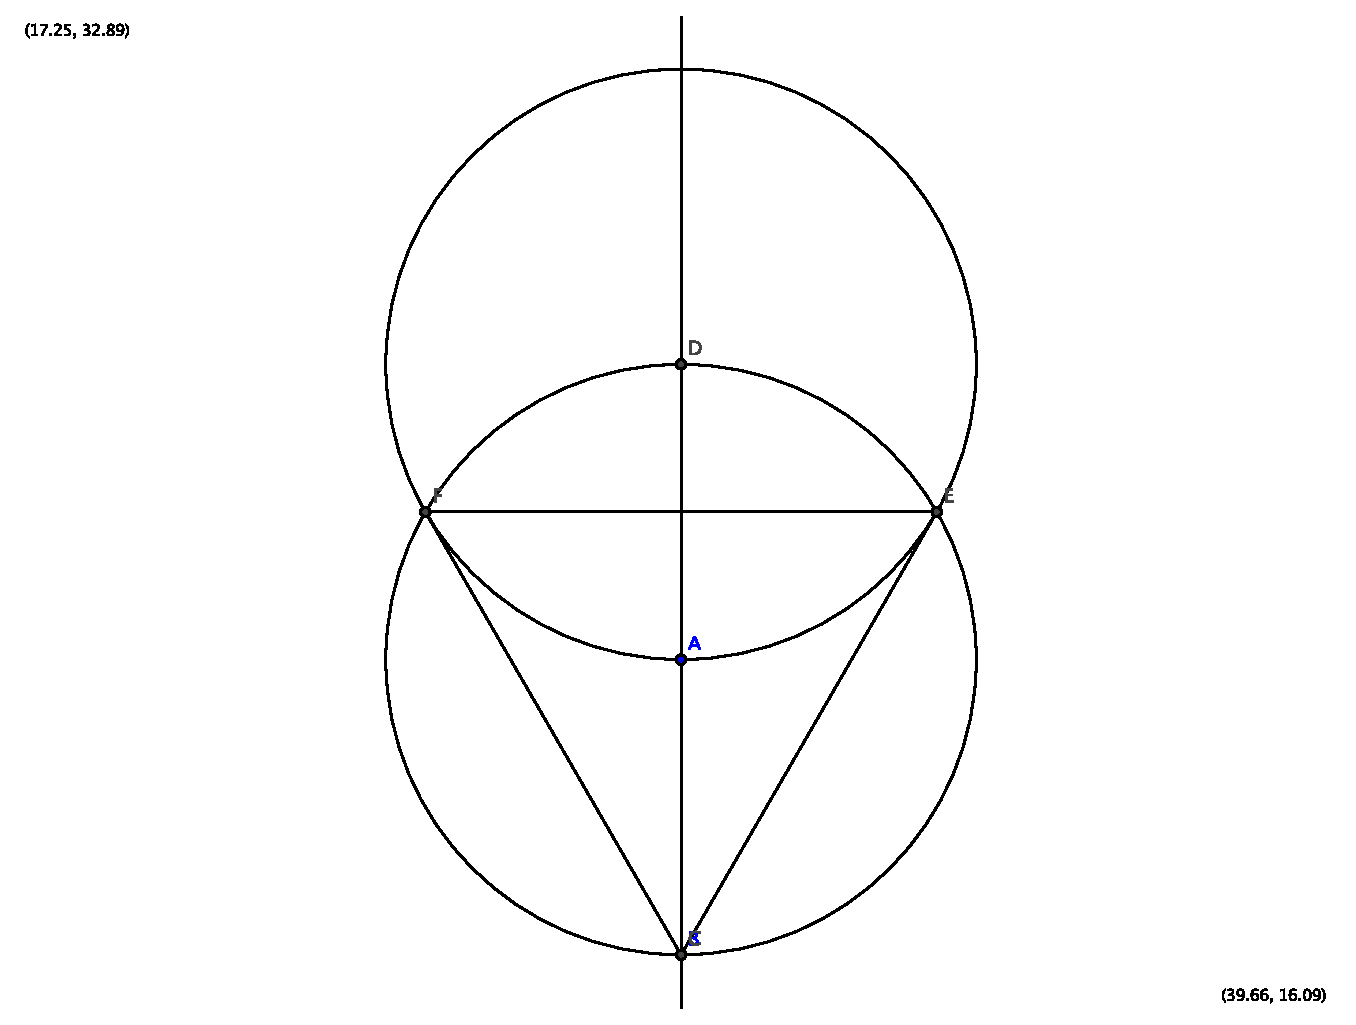
\includegraphics[scale=0.7]{\pathImages/Circles.eps}
\caption{Image instantiation (PDFs, vector, bitmap supported) }
\end{figure}


\section{In}
\subsection{ce}
\subsubsection{pt}
\subsubsubsection{ion}
\label{sssec:anion}

\newcommand{\yo} {
	\begin{flushright}
	\textit{Yo!} \begin{math}\times  \infty \end{math}
	\end{flushright}
}
\yo

%\include{Tex}
